\chapterimage{unidades/2_informacion/2_informatica/imagenes/cover}
\chapterimagedescription{Placa base de una computadora con sus circuitos impresos}
\chapterimageauthor{Fotografía de Blickpixel}

\chapter{Informática}

\setcounter{section}{4}
\section{Actividades}

\begin{exercise}
Valiendose de internet, determine para cada uno de los nombres completos de
archivo a continuación, de qué formato de archivo se trata (imagen, audio, texto,
programa ejecutable, etc.).

\begin{enumerate}[a)]
    \begin{minipage}{0.45\textwidth}
        \item ACDC.mp3
        \item bumbleebee.wav
        \item 2018\_06\_15\_221653.jpg
        \item logo.png
        \item index.php
        \item cv.docx
        \item materias.xls
        \item subtitles\_tbbt\_s01e04.zip
        \item script.sh
    \end{minipage}
    \begin{minipage}{0.45\textwidth}
        \item showcase.ppt
        \item cuadernillo.pdf
        \item day\_of\_the\_tentacle.exe
        \item LEEME.txt
        \item library.c
        \item configuration.xml
        \item run.py
        \item LEEME.md
        \item casa.dwg
    \end{minipage}
\end{enumerate}
\end{exercise}

\begin{enumerate}[a)]
    \item \textbf{ACDC.mp3} Un archivo de audio comprimido con codificación MP3.
    \item \textbf{LEEME.txt} Un archivo de texto plano
    \item \textbf{2018\_06\_15\_221653.jpg} Una imágen fotográfica con compresión JPEG.
    \item \textbf{run.py} Un archivo de texto plano con código Python.
    \item \textbf{index.php} Un archivo de texto que contiene código en lenguaje de programación PHP.
    \item \textbf{cv.docx} Un documento de Microsoft Word en su versión 2007 en adelante.
    \item \textbf{materias.xls} Un documento de Microsoft Excel en su versión previo a 2007.
    \item \textbf{subtitles\_tbbt\_s01e04.zip} Un archivo comprimido en formato ZIP.
    \item \textbf{script.sh} Un archivo de texto con código de scripting en BASH.
    \item \textbf{showcase.odp} Una presentación de diapositivas de Libre Office Impress.
    \item \textbf{cuadernillo.pdf} Un documento PDF.
    \item \textbf{day\_of\_the\_tentacle.exe} Un archivo ejecutable.
    \item \textbf{bumbleebee.wav} Un archivo de audo sin comprimir.
    \item \textbf{library.c} Un archivo de texto plano conteniendo código en lenguaje C.
    \item \textbf{configuration.xml} Un archivo de texto plano con código del lenguaje de marcado XML.
    \item \textbf{logo.png} Una imágen o dibujo con compresión PNG.
    \item \textbf{LEEME.md} Un archivo de texto plano con código del lenguaje de marcado Markdown.
    \item \textbf{casa.dwg} Un archivo de Autodesk AutoCAD.
\end{enumerate}
\vspace{1cm}

\begin{exercise}
Teniendo en cuenta el siguiente sistema de archivos de Windows que
corresponde a un DVD de una película, se pide.

\centerline{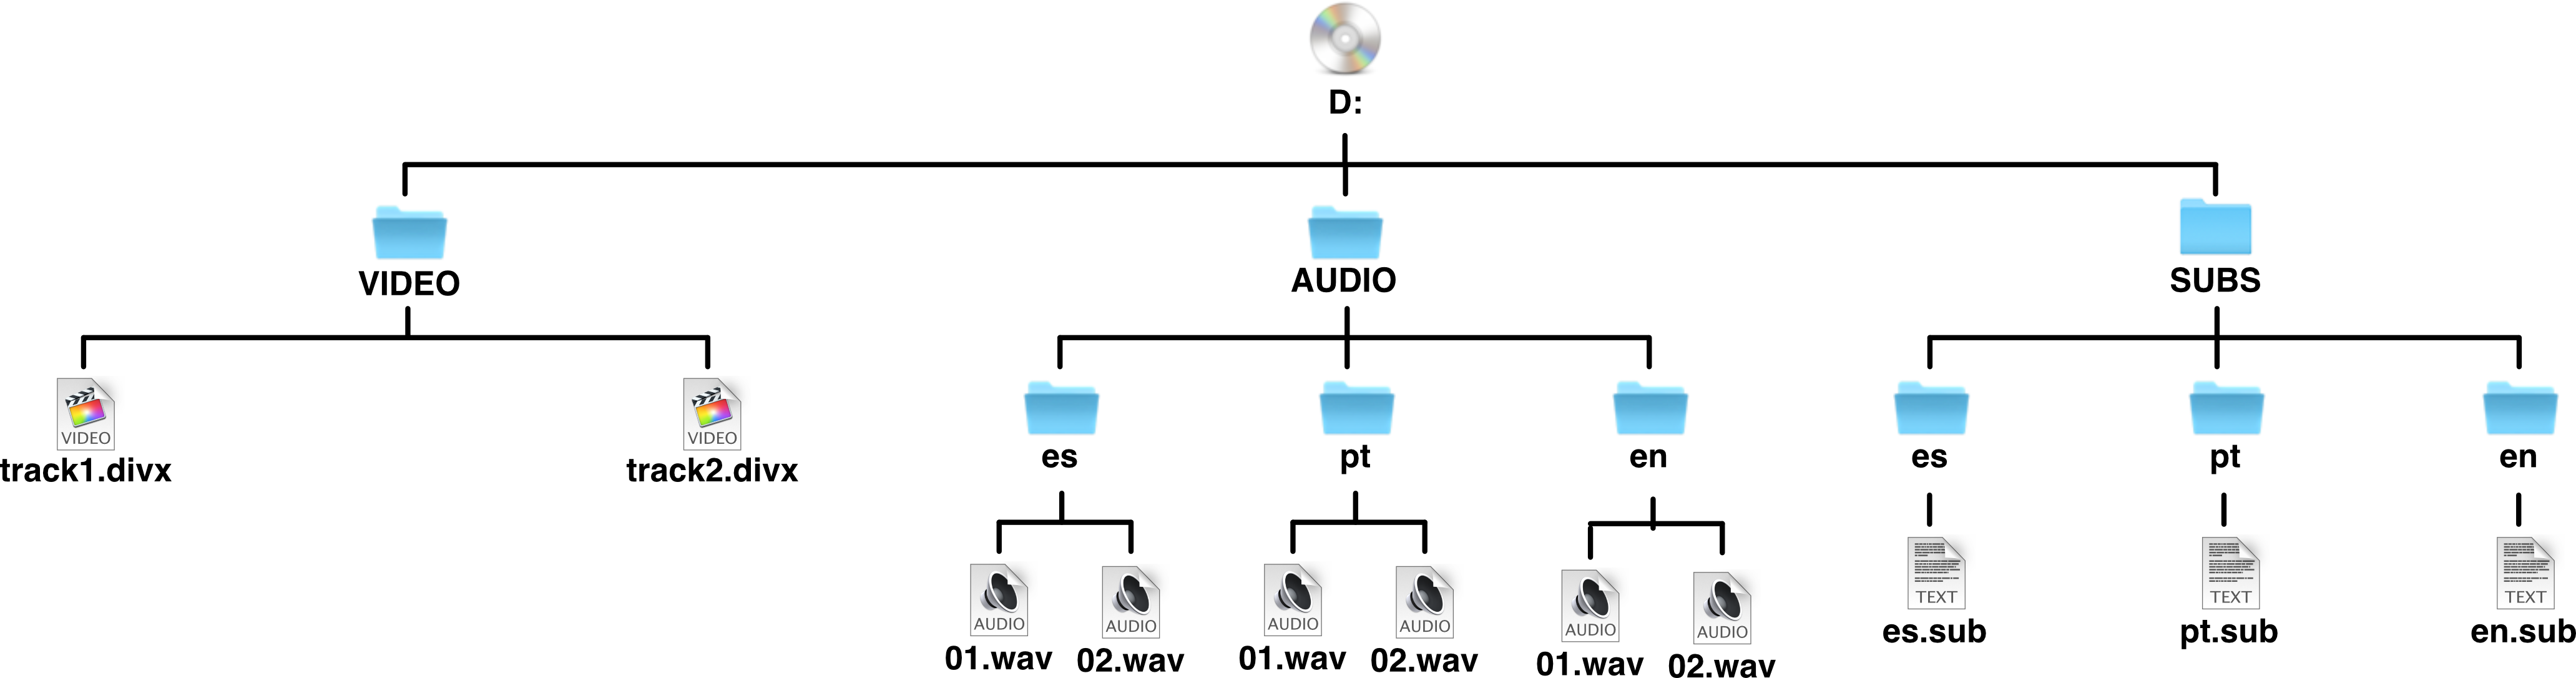
\includegraphics[scale=0.4]{unidades/2_informacion/2_informatica/imagenes/directorios_windows_4.png}}

Se pide que escriba las siguientes rutas absolutas:
\begin{enumerate}[a)]
    \item Al archivo de subtitulos en inglés (en.sub)
    \item Al archivo de audio de la pista 02 en español (carpeta es, archivo 02.wav)
    \item Al archivo de video de la pista 01 (track1.divx)
    \item Al archivo de audio de la pista 01 en portugues.
\end{enumerate}
\end{exercise}

\begin{enumerate}[a)]
    \item D:\textbackslash SUBS\textbackslash en\textbackslash en.sub
    \item D:\textbackslash AUDIO\textbackslash es\textbackslash 02.wav
    \item D:\textbackslash VIDEO\textbackslash track1.divx
    \item D:\textbackslash AUDIO\textbackslash pt\textbackslash 01.wav
\end{enumerate}
\vspace{1cm}

\begin{exercise}
Teniendo en cuenta el sistema de directorios del ejercicio anterior y
sabiendo qué:
\begin{itemize}
    \item Todo archivo de subtitulos pesa 500 KB.
    \item Los archivos de audio de la pista 01 pesan 5 MB.
    \item Los archivos de audio de la pista 02 pesan 25 MB, menos el de idioma
        portugués que pesa 27MB.
    \item El archivo de video de la pista 01 pesa 340 MB.
    \item El archivo de vide de la pista 02 pesa 660 MB.
\end{itemize}

Se pide determine las siguientes:
\begin{enumerate}[a)]
    \item Cuanto pesa la carpeta VIDEO
    \item Cuanto pesa la carpeta SUBS
    \item Cuanto pesa en total el disco D:
\end{enumerate}
\end{exercise}

Una carpeta pesa tanto como la suma de los elementos que contiene. El proceso
es recursivo, es decir, si una carpeta contiene un archivo y una sub-carpeta,
pesará tanto como lo que pesa el archivo y lo que pesan todos los archivos
dentro de la sub-carpeta.

\begin{enumerate}[a)]
    \item 340 MB + 660 MB = 1000 MB = \textbf{1 GB}.
    \item Cada carpeta en SUBS pesa 500 KB + 500 KB = 1000 KB = 1 MB.
        Las tres carpetas juntas pensan entonces \textbf{3 MB}.
    \item Son entonces 1000 MB de la carpeta VIDEO, sumado a los 3 MB de
        la carpeta de SUBS. A eso se le debe sumar la carpeta AUDIO, donde
        cada sub-carpeta pesa 25 MB + 25 MB = 50 MB, con la excepción de
        la carpeta pt que pesa 25 MB + 27 MB = 52 MB.
        El total de AUDIO es entonces 50 MB + 50 MB + 52 MB = 152 MB.
        El total del disco es entonces: 1000 MB + 3 MB + 152 MB = \textbf{1155 MB}.
\end{enumerate}
\vspace{1cm}

\begin{exercise}
Teniendo en cuenta la siguiente porción de un sistema de archivos de un
sistema Linux:

\centerline{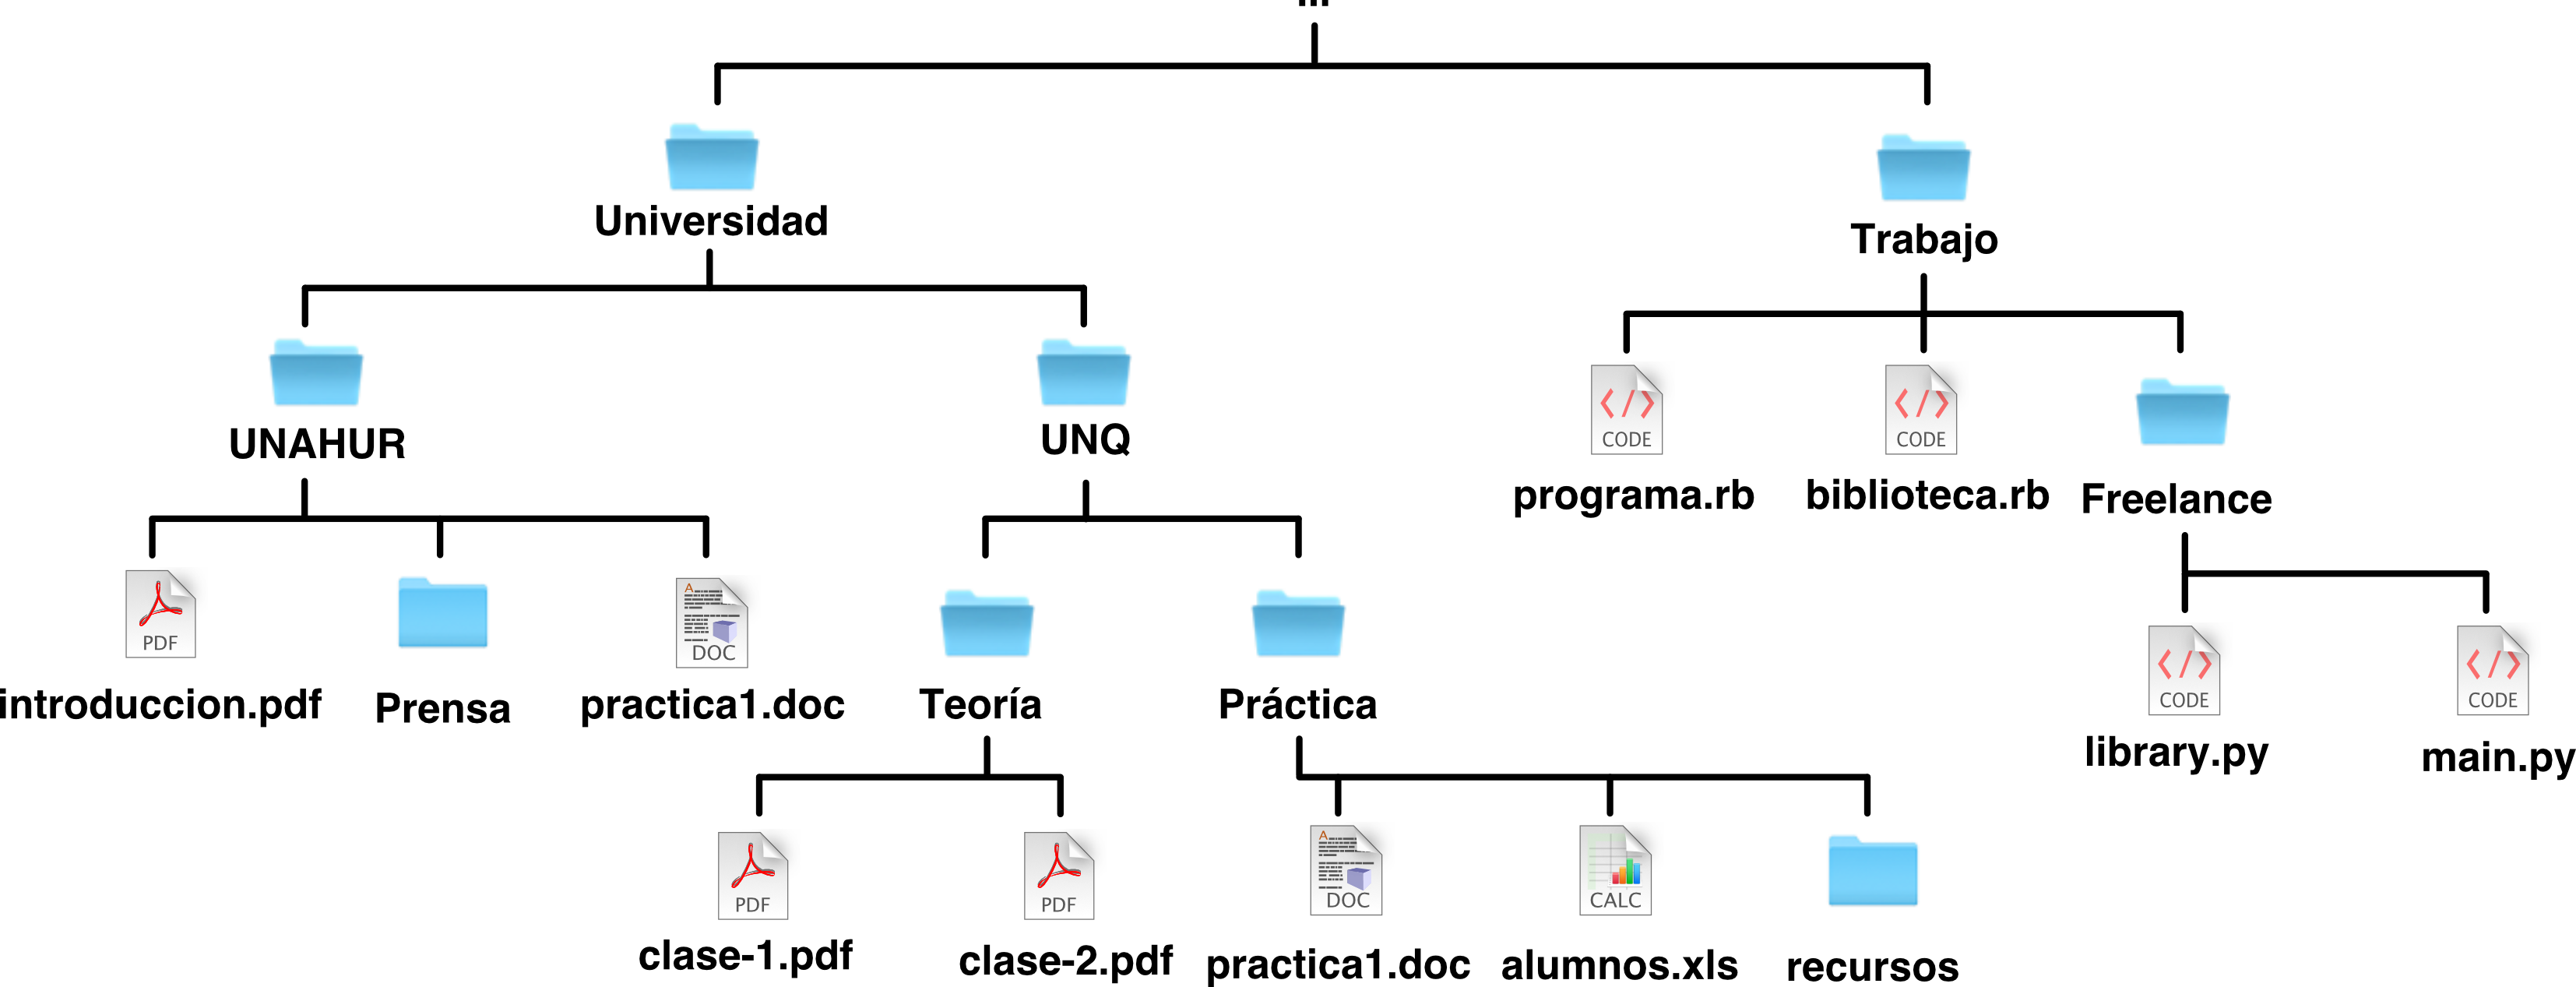
\includegraphics[scale=0.4]{unidades/2_informacion/2_informatica/imagenes/directorios_relativos.png}}

Describa la ruta absoluta a las carpetas que se encuentren vacías, asumiendo que la
carpeta superior es la raíz del sistema.
\end{exercise}

Solo se encuentran vacías las carpetas ``recursos'' y ``prensa''. Las rutas
asumiento que el inicio es la raíz del sistema son:

\textbf{/Universidad/UNAHUR/Prensa}

\textbf{/Universidad/UNQ/Práctica/recursos}

\vspace{1cm}

\begin{exercise}
Utilizando el mismo sistema de archivos del ejercicio anterior, escriba
las siguientes rutas relativas:
\begin{enumerate}[a)]
    \item Desde la carpeta más externa de la jerarquía hasta el archivo
        main.py
    \item Desde la carpeta más externa de la jerarquía hasta el archivo
        alumnos.xls
    \item Desde la carpeta UNQ hasta el archivo clase-2.pdf
    \item Desde la carpeta UNAHUR al archivo introduccion.pdf
    \item Desde la carpeta UNQ al archivo introduccion.pdf
    \item Desde la carpeta Teoría en UNQ al archivo programa.rb
\end{enumerate}
\end{exercise}

\begin{enumerate}[a)]
    \item Trabajo/Freelance/main.py
    \item Universidad/UNQ/Práctica/alumnos.xls
    \item Teoría/clase-2.pdf
    \item introduccion.pdf
    \item ../UNAHUR/introduccion.pdf
    \item ../../../Trabajo/programa.rb
\end{enumerate}

\vspace{1cm}

\begin{exercise}
Un programa ``hola mundo'' consiste en código que simplemente imprime en la
pantalla las palabras ``hola mundo''. Este tipo de programa se ha hecho popular
como una forma de poder dar a los programadores una vista minima y rápida de
la sintaxis de un lenguaje, y en cursos que se enfocan en la enseñanza de lenguajes
de programación en lugar de sus conceptos, es muy común encontrarlo como una de
las primeras muestras de código o actividades a realizar.

Se pide entonces que busque en internet el código de un programa ``hola mundo''
para los siguientes lenguajes de programación. Puede encontrar una gran colección
en el sitio \href{http://helloworldcollection.de}{http://helloworldcollection.de}

\begin{enumerate}[a)]
    \item Python
    \item Lisp
    \item C
    \item Java
    \item Assembly ARM
    \item Assembly z80, Console
\end{enumerate}

¿Qué reflexiones puede realizar despues de ver los diferentes códigos?
\end{exercise}

\vspace{0.5cm}
\noindent a) Python:
\begin{lstlisting}[language=python]
# Hola mundo en Python 2
print "Hola mundo"
\end{lstlisting}

\vspace{0.5cm}
\noindent b) Lisp:
\begin{lstlisting}[language=Lisp]
;;; Hola mundo en Common Lisp
(print "Hola mundo")
\end{lstlisting}

\vspace{0.5cm}
\noindent c) C:
\begin{lstlisting}[language=C]
/* Hola mundo en C */
#include <stdio.h>
#include <stdlib.h>

int main(void) {
    // La función main es el punto
    // de entrada del programa.
    puts("Hola mundo");
    return EXIT_SUCCESS;
}
\end{lstlisting}

\vspace{0.5cm}
\noindent d) Java:
\begin{lstlisting}[language=Java]
/* Hola mundo en Java */
// Mandatorio, todo el código debe estár
// siempre en una clase
class HelloWorld {
    // public static void main es el punto
    // de entrada del programa.
    public static void main( String args[] ) {
        // System.out contiene el stream de salida
        // al cual se le puede enviar el mensaje println
        System.out.println( "Hola mundo" );
    }
}

\end{lstlisting}

\vspace{0.5cm}
\noindent d) Assembly ARM
\begin{lstlisting}[language={[x86masm]Assembler},morekeywords={ldr,swi},morecomment={[s]{/*}{*/}}]
/*
    Hola mundo en Assembler para procesadores
    ARM (Dispositivos Android)
*/
.data

msg:
    .ascii      "Hola Mundo\n"
len = . - msg

.text

.globl _start
_start:
    mov     %r0, $1
    ldr     %r1, =msg
    ldr     %r2, =len
    mov     %r7, $4
    swi     $0
    mov     %r0, $0
    mov     %r7, $1
    swi     $0
\end{lstlisting}

\vspace{0.5cm}
\noindent e) Assembly z80, Consola
\begin{lstlisting}[language={[x86masm]Assembler},morekeywords={LD,CLEAR,DJNZ,JR,HALT,DEFB}]
; Este es un programa "Hola mundo"  para procesadores Z80 y
; TMS9918 / TMS9928 / TMS9929 / V9938 o V9958 VDP.
; Eso significa que debería funcionar en SVI, MSX,
; Colecovision, Memotech, y otras computadoras hogareñas
; y consolas de videojuegos basadas en el procesador Z80.
;
; Como no sabemos en que sistema va a funcionar, no sabemos
; donde está ubicada la memoria RAM, por lo que no podemos
; utilizar stack en este programa.
;
; Esta versión de "Hello World" fue escrita por
; Timo "NYYRIKKI" Soilamaa
; 17.10.2001
;
;----------------------------------------------------------------
; Configure esta parte:

DATAP: EQU #98 ; VDP Data port #98 funciona en todos los
; modelos MSX (TMS9918/TMS9929/V9938 or V9958)
; #80 funciona en SVI
; (para otras plataformas debería ver el manual y cargar esto)

CMDP: EQU #99 ; VDP Command port #99 funciona en todos los
; modelos MSX (TMS9918/TMS9929/V9938 or V9958)
; #81 funciona en SVI
; (para otras plataformas debería ver el manual y cargar esto)
;----------------------------------------------------------------
; El programa comienza acá:

ORG 0   ; El procesador Z80 comienza acá cuando se enciende
DI      ; No sabemos como funcionan las interrupciones en este
        ; sistema, por lo que las deshabilitamos.

; Configuremos la dirección de escritura de VDP a #0000
XOR A
OUT (CMDP),A
LD A,#40
OUT (CMDP),A

; Ahora limpiemos los primeros 16Kb de memoria VDP
LD B,0
LD HL,#3FFF
LD C,DATAP
CLEAR:
OUT (C),B
DEC HL
LD A,H
OR L
NOP     ; Esperemos ocho ciclos de reloj, solo en caso de
        ; que el VDP no sea lo suficientemente rápido
NOP
JR NZ,CLEAR

; Ahora es momento de configurar los registros del VDP:
;--------------------------------------------------------------
; Registro 0 a #0
;
; Poner el modo de selección del bit M3 (quizas también
; M4 y M5) en cero y deshabilitar el video externo e
; interrupciones horizontales
LD C,CMDP
LD E,#80

OUT (C),A
OUT (C),E
;--------------------------------------------------------------
; Registro 1 a #50
;
; Selecciona el modo de 40 columnas,
; habilita la pantalla y deshabilita las
; interrupciones verticales

LD A,#50
INC E
OUT (C),A
OUT (C),E
;--------------------------------------------------------------
; Registro 2 a #0
;
; Pone la tabla de patrones en #0000

XOR A
INC E
OUT (C),A
OUT (C),E
;--------------------------------------------------------------
; Registro 3 es ignorado en modo 40 columnas
; ya que no se requiere una tabla de colores
;
INC E
;--------------------------------------------------------------
; Registro 4 a #1
; Poner el patrón de generación de tablas en #800

INC A
INC E

OUT (C),A
OUT (C),E
;--------------------------------------------------------------
; Registros 5 (Atributos de sprites) y 6 (Patrones de
; sprites) son ignorados en modo de 40 columnas
; ya que este modo no tiene sprites

INC E
INC E
;--------------------------------------------------------------
; Registro 7 a #F0
; Pone los colores en texto blanco sobre fondo negro

LD A,#F0
INC E
OUT (C),A
OUT (C),E
;--------------------------------------------------------------

; Ponemos la dirección de escritura del VDP en #808
; de forma de poder escribir los caracteres en memoria
; (No hace falta escribir ESPACIO, ya es un caracter blanco)
LD A,8
OUT (C),A
LD A,#48
OUT (C),A

; Copiemos el juego de caracteres
LD HL,CHARS
LD B, CHARS_END-CHARS
COPYCHARS:
LD A,(HL)
OUT (DATAP),A
INC HL
NOP     ; Esperemos ocho ciclos de reloj, solo en caso de
        ; que el VDP no sea lo suficientemente rápido
NOP
DJNZ COPYCHARS

; Ponemos la direccion de escritura al comienzo de la tabla
XOR A
OUT (C),A
LD A,#40
OUT (C),A

; Ponemos los caracteres en pantalla
LD HL,ORDER
LD B,ORDER_END-ORDER
COPYORDER:
LD A,(HL)
OUT (DATAP),A
INC HL

JR OVERNMI
NOP
NOP

; Aquí está la dirección #66, es la entrada para NMI
RETN    ; Volver de NMI

OVERNMI:
DJNZ COPYORDER

; Fin
HALT

; Juego de caracteres:
; --------------------
ORDER:
DEFB 1,2,3,3,4,0,5,4,6,3,7
ORDER_END:

CHARS:

; H
DEFB %10001000
DEFB %10001000
DEFB %10001000
DEFB %11111000
DEFB %10001000
DEFB %10001000
DEFB %10001000
DEFB %00000000
; e
DEFB %00000000
DEFB %00000000
DEFB %01110000
DEFB %10001000
DEFB %11111000
DEFB %10000000
DEFB %01110000
DEFB %00000000
; l
DEFB %01100000
DEFB %00100000
DEFB %00100000
DEFB %00100000
DEFB %00100000
DEFB %00100000
DEFB %01110000
DEFB %00000000
; o
DEFB %00000000
DEFB %00000000
DEFB %01110000
DEFB %10001000
DEFB %10001000
DEFB %10001000
DEFB %01110000
DEFB %00000000
; W
DEFB %10001000
DEFB %10001000
DEFB %10001000
DEFB %10101000
DEFB %10101000
DEFB %11011000
DEFB %10001000
DEFB %00000000

; r
DEFB %00000000
DEFB %00000000
DEFB %10110000
DEFB %11001000
DEFB %10000000
DEFB %10000000
DEFB %10000000
DEFB %00000000
; d
DEFB %00001000
DEFB %00001000
DEFB %01101000
DEFB %10011000
DEFB %10001000
DEFB %10011000
DEFB %01101000
DEFB %00000000
chars_end:
\end{lstlisting}

Podemos ver que cada código es distinto, eso queda claro desde el primer momento.
Sin embargo, tambien podemos ver aquí que hay lenguajes que son de alto nivel,
y de bajo nivel. En los lenguajes de alto nivel, como Python o Lisp, el código
refleja más claramente la intención del programador. En los lenguajes intermedios,
como C, el código sigue reflejando de alguna forma la intención, pero empiezan a
aparecer elementos de sintaxis que se vuelven obligatorios, y que no aportan a
lo que uno quiere lograr. Java, por ser un lenguaje orientado a objeto, y ser
fuertemente tipado, solicita un monton de pasos protocolares simplemente para
poder escribir algo en pantalla (claramente no es un lenguaje pensado para tal
fin). Los Assembly ya nos resultan esotéricos, y uno debe conocer muy bien el
procesador, los chips de los equipos, y entender como se carga el programa en
la memoria. En ARM, si bien extraño, uno puede ver un ``Hola mundo'' escrito
en algún lado, en el de z80, solo aparecen ceros y unos en una tabla que refleja
los pixeles de la pantalla (cuales estarán prendidos y cuales apagados), indicando
el texto ``hello world''.

Una cosa interesante en el caso de Java, pero mucho más patente en el caso del
z80, es que los programadores dejan mensajes para otros seres humanos, y que no
son parte del programa mismo. Estos mensajes se llaman ``comentarios''. El
código del z80 es tan extraño a lo que uno quiere hacer realmente, que requiere
una gran cantidad de comentarios para reflejar la idea que el programador tenía
en la cabeza. Si quitamos los comentarios de ese programa, sería muy dificil
(casi imposible) comprender qué ese programa es un ``hola mundo''. Es importante
que el código transmita ideas, y no solo que funcione, si el código funciona pero
no se entiende, no podrá ser compartido. Peor aún, no podrá ser mantenido en el
tiempo, ni siquiera por el mismo programador, pues este olvidará qué es lo que
escribió con el tiempo.
\vspace{1cm}

\begin{exercise}
El sitio web \href{https://alternativeto.net}{https://alternativeto.net} permite
a sus usuarios buscar un programa por nombre, y brinda alternativas a ese programa
con funcionalidades equivalentes o similares. Dentro de los resultados, se puede
filtrar por sistema operativo y por el tipo de licencia (comercial, gratuita o libre).

Se pide que busque al menos una alternativa que sea software libre y/o open
source para cada uno de los siguientes programas:
\begin{enumerate}[a)]
    \item Windows 10
    \item Microsoft Office Suite
    \item Adobe Acrobat Reader
    \item Internet Explorer
    \item Adobe Photoshop
    \item Autodesk AutoCAD
    \item Age of Empires II
\end{enumerate}
\end{exercise}

\noindent a)

En general cualquier distribución de Linux o de BSD es una alternativa.
Algunas están más asentadas y por tanto, son de mejor calidad que otras,
pero pueden encontrarse alternativas, no solo a Windows 10, sino a cualquier
otra versión de Windows, con distribuciones pensadas para correr en
máquinas antiguas o de baja potencia, en tablets, etc.

Algunas de las alternativas son:
\begin{enumerate}
    \item \textbf{Ubuntu}
    \item \textbf{Linux Mint}
    \item \textbf{Debian}
    \item \textbf{Fedora}
    \item \textbf{ZorinOS}
\end{enumerate}

\noindent b)

\begin{enumerate}
    \item \textbf{LibreOffice}\\
        LibreOffice surge como un derivado de OpenOffice. A diferencia de este
        último utiliza una licencia GPL, por lo que se código no puede ser objeto
        de productos comerciales. Por eso, se ha transformado en la suite por
        defecto de la mayoría de las distribuciones Linux.
    \item \textbf{Apache OpenOffice}\\
        OpenOffice nació como una suite ofimática libre de la mano de la empresa
        Sun Microsystems. Cuando Sun fue adquirida por Oracle Corporation, los
        usuarios temieron que Oracle cerrara la rama de desarrollo de OpenOffice,
        algo que efectivamente sucedió. La fundación Apache se hizo cargo de
        OpenOffice, pero en el caótico proceso nació también LibreOffice.
    \item \textbf{Calligra}\\
        Calligra es una suite compuesta por aplicaciones tanto de ofimática,
        como de diseño gráfico. Es un conjunto de aplicaciones de KDE, por lo
        que viene instalado en muchas distribuciones Linux que utilizan ese
        entorno.
\end{enumerate}

\noindent c)

En general cada distribución de Linux incluye uno. Hoy en día también Google
Chrome y Firefox incluyen lector de PDF integrado, y su código es libre.
\begin{enumerate}
    \item \textbf{Sumatra PDF}\\
        Diseñado para Windows como una alternativa libre.
    \item \textbf{Evince}\\
        Lector por defecto en los sistemas Linux que utilizan el escritorio GNOME.
    \item \textbf{Okular}\\
        Lector por defecto en los sistemas Linux que utilizan el escritorio GNOME.
\end{enumerate}

\noindent d)

\begin{enumerate}
    \item \textbf{Mozilla Firefox}\\
        Firefox existe desde hace ya muchos años como competencia de IE.
        Nació como una continuación del proyecto comercial Netscape, el cuál
        abrió su código tras dar quiebra la empresa. Hoy en día es una de las
        alternativas más elegidas entre los usuarios de software libre.
    \item \textbf{Google Chromium}\\
        Chromium es el proyecto libre de donde se produce Google Chrome
        (que agrega unas pocas caracteristicas no libres al mismo). Surgió
        en Google con la intención de fomentar el uso de la web moderna y
        plantar una seria competencia a IE
\end{enumerate}

También existen muchas otras alternativas más pequeñas y menos populares.

\noindent e)

\begin{enumerate}
    \item \textbf{GIMP}\\
        Es ``él'' editor libre. Posee gran cantidad de caracteristicas avanzadas
        y una gran base de usuarios, tutoriales, foros, etc.
    \item \textbf{Krita}\\
        Krita es el editor por defecto en sistemas de escritorio KDE.
    \item \textbf{Pinta}\\
        Una alternativa libre en Windows, diseñada a partir del código de Paint.NET,
        posee caracteristicas avanzadas, y una buena base de usuarios.
\end{enumerate}

\noindent f)

En general, si bien hay alternativas libres, están muy atrás con respecto a
la alternativa privativa en este area. Algunas opciones son:
\begin{enumerate}
    \item \textbf{FreeCAD}
    \item \textbf{LibreCAD}
    \item \textbf{OpenSCAD}
\end{enumerate}

\noindent g)

Existen diferentes alternativas de juegos similares a AoE II, muchas con baja
calidad. Cabe mencionar el proyecto, aún en desarrollo pero con una excelente
calidad y potencial, 0 A.D.
\begin{enumerate}
    \item \textbf{0 A.D.}
    \item \textbf{MegaGlest}
    \item \textbf{Widelands}
\end{enumerate}